\documentclass[10pt,twocolumn]{article}
\usepackage{graphicx}    % For including images
\usepackage{amsmath}     % For mathematical symbols
\usepackage{caption}     % Better captions
\usepackage{float}       % Precise float placement
\usepackage{geometry}    % To adjust margins
\geometry{margin=1in}
\usepackage[backend=biber,style=apa]{biblatex}
\addbibresource{references.bib}  % This is your .bib file name

\title{\textbf{Machine Learning-Based Classification of Table Tennis Swings Using Racket Kinematics}}
\author{Jevi Waugh \\
Faculty of Engineering, Architecture and Information Technology \\
COMP4702 - Machine Learning}
\date{May 2025}

\begin{document}

\maketitle
% START OF PAGE 1
\begin{abstract}
This report investigates the application of machine learning models to classify the demographics of table swings based on racket kinematics data, with a strong focus on predicting a combined age and gender label. The Data Set originally sourced from DRYAD has slightly been modified for the purpose of this report. We apply and compare three supervised classification algorithms, K-Nearest Neighbours (KNN), Support Vector Machines (SVM) and One-vs-Rest Logistic Regression, evaluating their performance using known evaluation metrics. Our findings provide insights into the discriminative power of racket motion features and the behaviour of various classifiers on a real-word problem. 
\end{abstract}
%
\section{Introduction}
Human motion analysis and dexterity is a core area of research in sports, particularly in table tennis. In the context of table tennis, it is important to understand how swing patterns relate to certain demographic attributes such as age and gender, which can inform training strategies and biomechanical insights such as angular velocity, acceleration, power spectral density, etc. This report explores the use of supervised machine learning models to classify a composite label consisting of age and gender from the table tennis-racket-swing dataset. Pre-Processing will be required to ensure that valid numerical data are utilised efficiently. The considered ML models: K-Nearest Neighbor (K-NN), logistic regression and kernel based methods (such as a support vector machine) will be used. The purpose of this report is not to only maximise accuracy and lower $E_{new}$, but to primarily make a critical evaluation of each model's behaviour, generalisation capability, feature processing, and sensitivity to hyper-parameters.

\section{Exploratory Data Analysis}
The provided dataset had some irregularities in terms of feature values and also had other inconsistencies with our classification task. The features that were dropped are 'id' and 'date' primarily because ID identifies and metadata impertinent to the player kinematics will strictly skew the classification workflow as they are strictly not-relevant to the problem.
\subsection{Encoding and Normalisation}
Our classification problem will make use one-hot-encoding for features in Table~\ref{tab:cat-values} excluding "???".  Age encodes,  low $\rightarrow$ 0, medium $\rightarrow$ 1, high $\rightarrow$ 2. This provides us the following 6 labels as shown in Table~\ref{tab:encoding-scheme}. 
We then represent these modalities as low $\rightarrow$ Young, medium $\rightarrow$ Mid-age, high $\rightarrow$ Older.
For gender, we have binary numerical values which we interpret as, 0 $\rightarrow$ Female, and 1 $\rightarrow$ Male. 
\footnote{Note that Gender is interpreted, not encoded; age is encoded once, then interpreted via standard terms.}
\begin{table}[H]
\centering
\caption{Encoding scheme for combined gender and age classification}
\begin{tabular}{|l|}
\hline
\textbf{Combined Labels} \\
\hline
00 $\rightarrow$ Young Female \\
10 $\rightarrow$ Young Male \\
01 $\rightarrow$ Mid-age Female \\
11 $\rightarrow$ Mid-age Male \\
02 $\rightarrow$ Older Female \\
12 $\rightarrow$ Older Male \\
\hline
\end{tabular}
\label{tab:encoding-scheme}
\end{table}
The dataset will be either normalised using the formula \begin{equation}x_{ij}^{new} = {\dfrac {x_{ij} - min_l{(x_{lj})}} {max_l{(x_{lj})} - min_l{(x_{lj})}}}\label{eq:minmax}
\end{equation} or standardised, using   $Z={\dfrac {\bar{X} - \mu} {\sigma}}$depending on the model's sensitivity to feature scaling and the distribution of the data.
\subsection{Dataset description and assumptions}
\label{subsec:dataset-description-and-assumptions}
The dataset has 97,355 data-points \footnote{Modified data from source \cite{dryad_tabletennis2021}.} and 49 features excluding 'id' and 'date'. There were other inconsistencies such as missing values labelled as "???" in certain columns (see Table~\ref{tab:cat-values}). There were 5 missing data points in each random variable (feature), 20 values, a total of which their rows were dropped. We also assume that the dropped rows won't affect prediction accuracy given that its only $5.13 \times 10^{-5}$\% of the entire data set.

\begin{table}[H]
\centering
\caption{Categorical values (before cleaning)}
\begin{tabular}{|l|l|}
\hline
\textbf{Feature} & \textbf{Unique Values} \\
\hline
Height     & \texttt{high, low, medium, ???} \\
Age        & \texttt{high, medium, ???, low} \\
Play Years & \texttt{high, medium, ???, low} \\
Weight     & \texttt{high, medium, low, ???} \\
\hline
\end{tabular}
\label{tab:cat-values}
\end{table}
Furthermore, an analysis on class imbalance was made to ensure full interpretability when we make predictions. We can see that in Figure~\ref{fig:stacked-results} gender has a class imbalance of 60-40\%.To address the class imbalance in gender, we will use the stratify parameter in Scikit-learn's \texttt{train\_test\_split}
 function to ensure that proportion of each class is preserved in both the training and test sets. Without stratification, random splitting of the data might over-represent one class leading to a biased model. While this imbalance is not as extreme as  presented ones such as Figure~\ref{fig:stacked-hand-results}, this ensures a much more accurate model. \texttt{Handedness} and \texttt{holdRacketHanded} both have an exact imbalance of 83-16\%. We will address this later during feature selection. 

\begin{figure}[H]
    \centering
    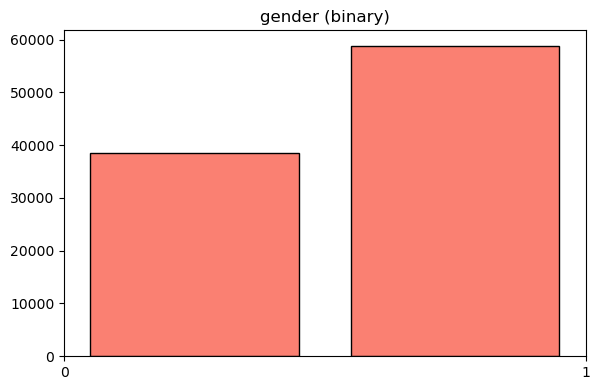
\includegraphics[width=0.85\linewidth]{images/gender.png}
    \caption{Gender Imbalance}
    \label{fig:stacked-results}
\end{figure}

\begin{figure}[H]
    \centering
    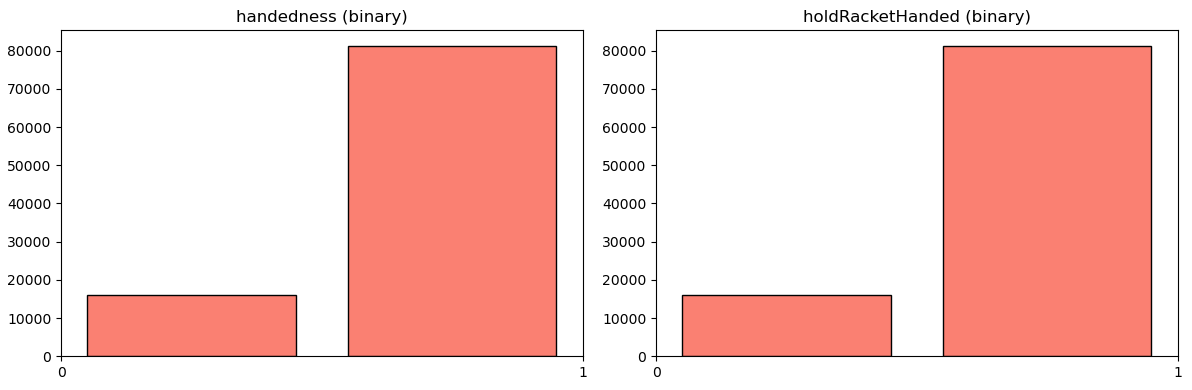
\includegraphics[width=0.85\linewidth]{images/hand_data.png}
    \caption{Hand data Imbalance}
    \label{fig:stacked-hand-results}
\end{figure}

We also observe the distributions of each numerical feature in the figures in the appendix. While some features exhibit skewness and uniformity, many including \texttt{newv1}, \texttt{newv2} and \texttt{g\_max} appear to follow a roughly Gaussian distribution. Although strict normality cannot be assumed without some sort of formal statistical testing, we proceed under the simplifying assumption that the data is normally distributed.  The Central Limit Theorem suggests that convergence to a Gaussian distribution as $n \rightarrow \infty $, even when the underlying data is not perfectly Gaussian.\footnote{For intuition, imagine the histogram having smaller bin widths—this would clarify whether the distribution approximates a known form.}
 This is considered a reasonable assumption for the purposes of standardisation and model compatibility.

Before applying any machine learning model, we will identify potential redundancy among features by computing a Pearson correlation matrix as seen in Figure~\ref{fig:correlation-matrix}
\begin{figure}[H]
    \centering
    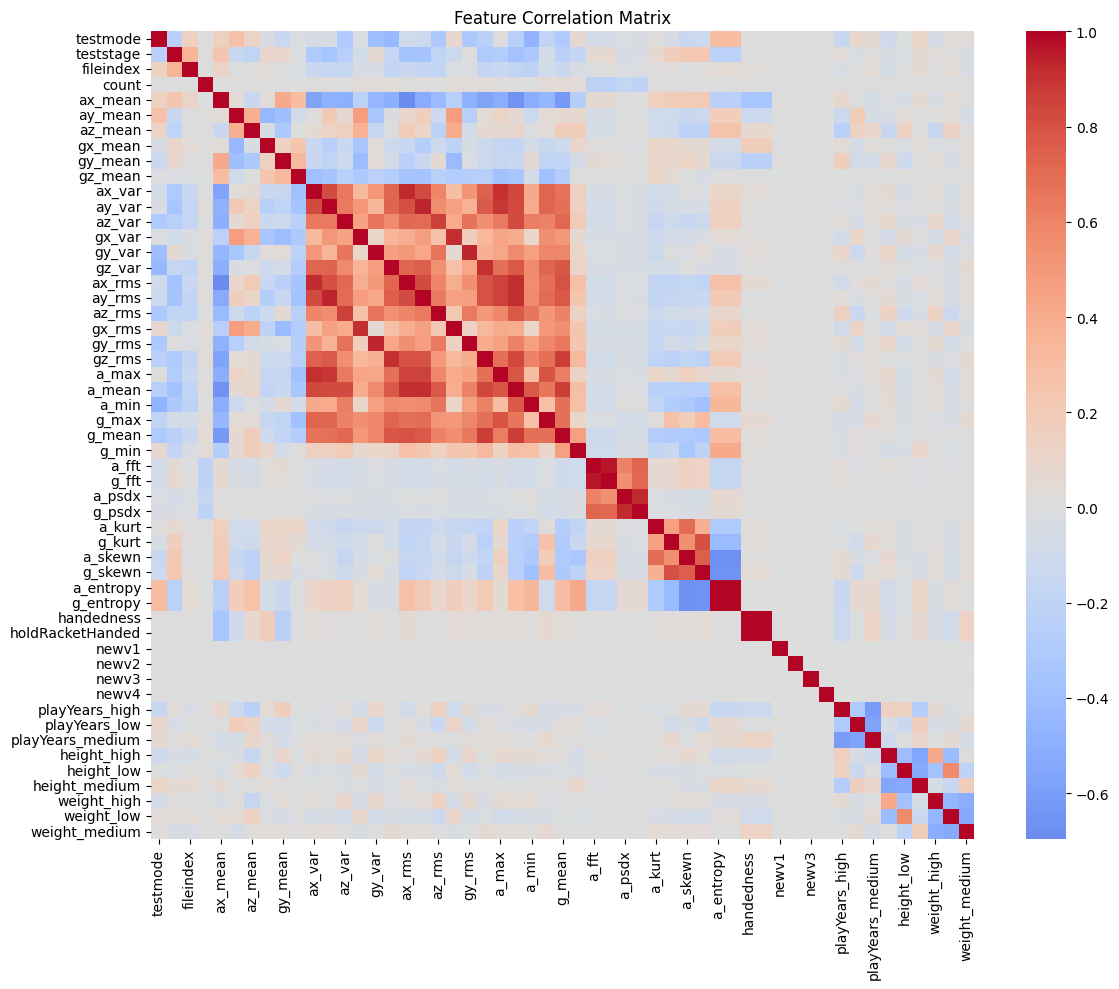
\includegraphics[width=0.85\linewidth]{images/correlation_matrix.png}
    \caption{Pearson's correlation matrix}
    \label{fig:correlation-matrix}
\end{figure}
We can see that the acceleration, velocity and gyro-signal features are heavily correlated. Highly correlated features can introduce multicollinearity which can negatively impact a model that assumes feature independence (such as Logistic regression). Dropping highly correlated features will be further explored in other models to evaluate its effectiveness and generalisation.
% START OF PAGE 2
\section{Model 1: K-Nearest Neighbours (KNN)}
We will first explore K-Nearest neighbour as it's a non-parametric model that uses the euclidean distance metric. We will also discuss how normalisation and this distance metric simultaneously affect the accuracy.
\subsection{Model Training and Hyper-parameter tuning}

From an experimentation perspective, we will normalise instead of standardise to see how the model operates disregarding our initial assumption about the distribution of the data. First we train an initial model with \texttt{K=1, K=3}, requiring approximately 5 minutes of computation time during model training and with an 80/20 train-test split, reserving 20\% of the data for testing. This resulted into a classification accuracy of 53\% and 63\% respectively. Empirically speaking, we observed (based on the distribution of the random variables) that when features are skewed or contain outliers, normalisation compresses the majority of the data into a narrow range, which distorts the euclidean calculations and leads to reduced performance. This is another reason why our model focuses more on using the $z-score$ while normalisation fails Equation~\ref{eq:minmax}.

Now suppose we standardise as we are meant to, which reduces the effect of differing feature scales and we apply the same conditions as before but for different $k$ values as outlined in Figure~\ref{fig:knn-k}.


\subsection{Accuracy and classification}
After model training and finding the optimal $k$ value based on the lowest $E_{new}$ in Figure~\ref{fig:knn-k}, we see high performance across all classes, with precision, recall, and F1-scores averaging around 96-97\%. The accuracy for training was 98\% while the test data set yielded 96\%. The confusion matrix in Figure~\ref{fig:knn-cm} confirms this, displaying strong diagonal dominance, especially for the two most accurate class 1-0 (Young Male) and 1-2 (Older Male), which achieved 1588 out of 1640, and 5849 out of 6060 correct predictions respectively. Minor off-diagonal entries suggest that misclassifications tend to occur between adjacent classes, likely due to overlapping feature distributions (e.g., confusion between 0-0 and 0-2 or between 1-1 and 1-2). This is expected in a demographic classification task where class boundaries may be gradual. 

\begin{figure}[H]
    \centering
    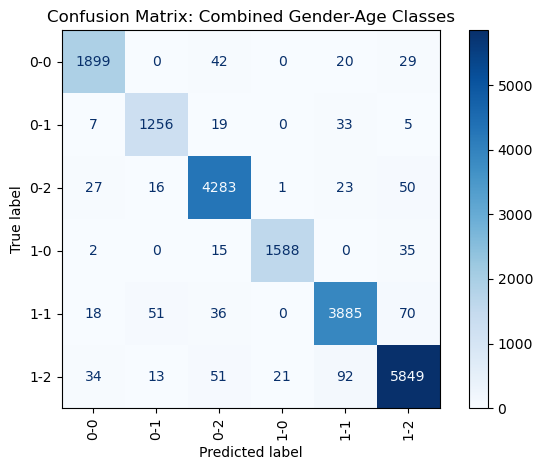
\includegraphics[width=0.85\linewidth]{images/knn/knn cm.png}
    \caption{KNN Confusion Matrix}
    \label{fig:knn-cm}
\end{figure}
Analysing scores in lower support classes such as class 1 (1320 samples) and class 3 (1640 samples) indicate that the model is not overfitting to the majority classes. Moreover, if we look deeper, there are about 70 instances (in Figure~\ref{fig:knn-cm}) of class 1-1 (Mid-age Male) confused with 1-2 (Older Male). Our argument to this is the inherent ambiguity in defining discrete age categories based on continuous physiological behaviour. There is no clear margin for what constitutes "mid-age" and "older", and swing kinematics in terms of angular velocity in all axes when using the racket could be very similar. For example, if the age cutoff for "mid-age" is 55 and the and "Older" began at 56, then individuals close to that threshold would likely produce nearly indistinguishable kinematic patterns. This could very well result in a very similar feature distribution. Hence, while class "medium" and "high" may signify the age of an individual, the model does not take into account, that they could potentially represent similar feature patterns near boundary ages.
%
\begin{table}[H]
\centering
\small  % Reduce font size
\caption{Classification report for 6-class model}
\resizebox{\linewidth}{!}{%
\begin{tabular}{lcccc}
\hline
\textbf{Class} & \textbf{Precision} & \textbf{Recall} & \textbf{F1} & \textbf{Support} \\
\hline
0 & 0.96 & 0.95 & 0.95 & 1990 \\
1 & 0.94 & 0.95 & 0.95 & 1320 \\
2 & 0.96 & 0.97 & 0.97 & 4400 \\
3 & 0.99 & 0.97 & 0.98 & 1640 \\
4 & 0.96 & 0.96 & 0.96 & 4060 \\
5 & 0.97 & 0.97 & 0.97 & 6060 \\
\hline
\textbf{Accuracy} & \multicolumn{3}{c}{0.96} & 19470 \\
\textbf{Macro Avg} & 0.96 & 0.96 & 0.96 & 19470 \\
\textbf{Weighted Avg} & 0.96 & 0.96 & 0.96 & 19470 \\
\hline
\end{tabular}
}
\label{tab:classification-report}
\end{table}

In Table~\ref{tab:classification-report}, we can see the Macro avg and weighted all around around 0.96 suggesting consistent performance and reliable generalisation, given class imbalance present in the dataset was handled.
% START OF PAGE 3
\clearpage  % or \newpage
The Figure~\ref{fig:knn-k} illustrates the test error $E_{new}$ across various $k$ values in the classifier. This was done iteratively with random sampling and tuning this $k$ hyper-parameter really showed certain drops in accuracy although the differences were not more than 0.01. A sharp drop is observed at $k=3$, which achieves the lowest test error 3.65\%, along with $k=5$ suggesting a good balance between bias and variance since their training accuracies were both 98\% which is close to 2\% higher than their test accuracy 96\%.  In this case, we choose $k=3$.
\subsubsection{$E_{new}$ evaluation}
\begin{figure}[H]
    \centering
    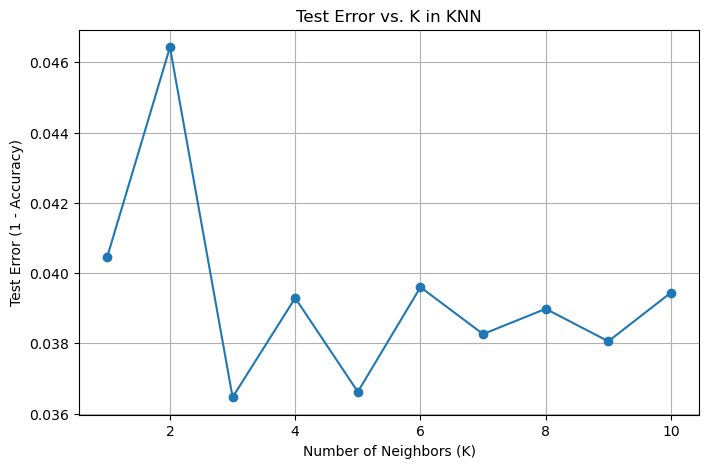
\includegraphics[width=0.85\linewidth]{images/knn/knnn k's.png}
    \caption{$E_{new}$ for each $k$}
    \label{fig:knn-k}
\end{figure}
As $K$ increases, the errors fluctuates but remain relatively low, suggesting that the model is stabilising beyond $k=3$. This supports the idea that selecting an appropriate $K$ value is crucial as very small $k$ or very large $k$ can affect the model's performance. Furthermore, the magnitude of $K$ is not the only thing that affects the classifier, but considering whether $K$ is odd or even. Using an odd $K$ helps reduce the likelihood of tied votes when classifying. Although ties are less common in a six-class problem compared to binary classification, they can still occur, especially when boundary samples are surrounded by neighbours from different classes. Figure~\ref{fig:knn-k} is an illustration of this effect where every even $k$ value is higher than the odd values next to it.
\subsection{Evaluation Metrics and Results}
We will perform a deeper evaluation using an ROC curve and the learning curves of training and testing through different batches of the hold-out validation data.WRITE MORE
\subsubsection{ROC Curves}
The ROC curve in Table~\ref{fig:knn-roc} was computed using the one-vs-rest approach for each class showing perfect AUC scores of 0.99 across almost all classes except class 1-0 which achieves 1.0. While this looks suspicious, let's understand that this has a connotation of KNN's strong ability to differentiate between classes, it is important to note that these high score only measure how well the model separates the classes and not whether it assigns the correct label and may still misclassify samples when forced to make difficult predictions as outlined on page 3 when classifying between "Mid-age Male" and "Older Male" etc...
\begin{figure}[H]
    \centering
    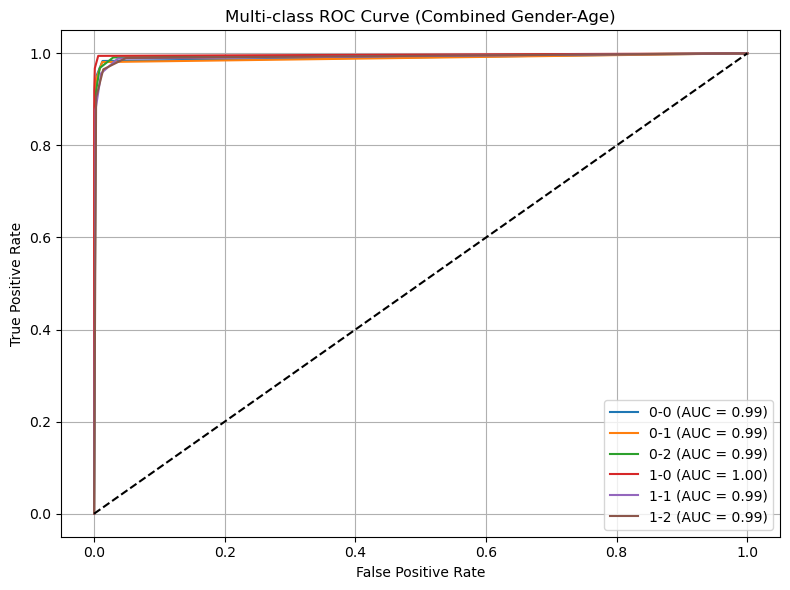
\includegraphics[width=0.85\linewidth]{images/knn/roc curve.png}
    \caption{KNN ROC Curve.}
    \label{fig:knn-roc}
\end{figure}

Although stratified sampling was used, class imbalance remains a fundamental characteristic. When evaluating using one-vs-rest ROC curves, larger classes such as 1-2 in Table~\ref{tab:combined-class-distribution} dominates the score computations and classifiers generally do better if they have more examples to learn from. In terms of the AUC bias, it seems that for KNN's result that, it's easier to get a high AUC for large classes, regardless if the precision, F1 or even the recall metric is worse for classes with less examples.

\begin{table}[H]
\centering
\caption{Distribution of Combined Gender-Age Classes}
\begin{tabular}{|c|c|}
\hline
\textbf{Class (Gender-Age)} & \textbf{Count} \\
\hline
1-2 (Male–High)   & 30,300 \\
0-2 (Female–High) & 22,000 \\
1-1 (Male–Medium) & 20,300 \\
0-0 (Female–Low)  & 9,950 \\
1-0 (Male–Low)    & 8,200 \\
0-1 (Female–Medium) & 6,600 \\
\hline
\end{tabular}
\label{tab:combined-class-distribution}
\end{table}
It is critical to make the observation that there are significantly less young people than "mid-age" and "older" people.

\clearpage  % or \newpage
\subsubsection{Cross validation and learning curve}
We do another form of experimentation to see if our previous results hold, by strictly evaluating the performance of KNN with an initial 5-fold cross in Table~\ref{tab:cv-scores} with $k=3$ across the entire dataset. The resulting accuracy scores showed moderate variance across folds, with a mean accuracy of approximately 54.7\%.This is not ideal but we understand that this is also due to the fact that there was no \texttt{stratify} parameter in sci kit-learn's \texttt{cross\_val\_score} function not directly handling the class (combined label) imbalance.
\begin{table}[H]
\centering
\caption{5-Fold Cross-Validation Accuracy Scores}
\begin{tabular}{lc}
\hline
\textbf{Fold} & \textbf{Accuracy} \\
\hline
1 & 0.572 \\
2 & 0.626 \\
3 & 0.628 \\
4 & 0.478 \\
5 & 0.431 \\
\hline
\textbf{Mean} & \textbf{0.547} \\
\hline
\end{tabular}
\label{tab:cv-scores}
\end{table}
While KNN evaluates each fold, it's strongly suspected that these accuracies are strictly modest due to the concentration of similar-class samples within individual folds.  This is problematic as we can see in Table~\ref{tab:combined-class-distribution}, classes such as 1-2 dominate while 0-1 are underrepresented. This limited diversity significantly lowers $E_{hold-out}$ in each fold reducing the model's ability to generalise.

\begin{figure}[H]
    \centering
    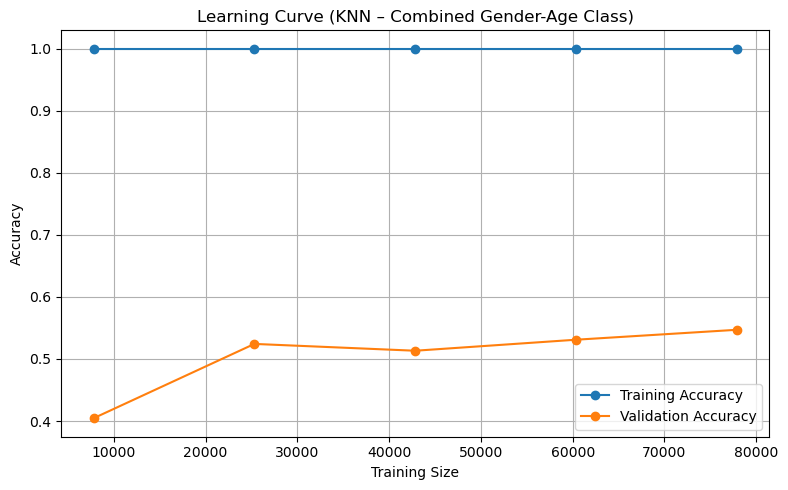
\includegraphics[width=0.85\linewidth]{images/knn/learning rate and cross validation.png}
    \caption{KNN Learning curve}
    \label{fig:knn-lrate}
\end{figure}
We analyse the learning curve of KNN generated using 5-fold cross validation providing increase in accuracy for varying training sizes. For training accuracy, it's not surprising to see KNN memorising the data resulting in 100\%. However the validation accuracy for each training batch plateaus around 55\% even though it increases every time the training size increases. Although this gradual rise indicates that the model benefits from more data, the persistent gap between training and validation performance shows that there is an immense amount of high variance and overfitting. Unlike the previous split cross validation approach shown in Table~-\ref{tab:cv-scores}, this cross-validated method approach offers a more robust estimate of KNN's true capabilities as a model that primarily looks at local neighbourhood structures in the data. Since it has a big generalisation gap, it's fair to say that KNN struggles to generalise well in high-dimensional, imbalanced multi-classification problems. 

This conclusion is made primarily because of KNN's inherent sensitivity to class imbalance class imbalance and because hold-out cross-validation forces the model to generalise over all parts of the data in terms of varying class distributions.  A more complex model is required to improve generalisation for our high-dimensional dataset.

% START OF PAGE 4
% \clearpage  % or \newpage
\section{Model 2: Logistic regression}
Unlike KNN, logistic regression is a parametric model that learns a set of weights $\theta$ to separate classes using linear decision boundaries using the logistic loss~\ref{eq:logistic-loss}

\subsection{Solver and regularisation analysis}
Training logistic regression took a significant amount of time (1H+) to compute and we had the same initialisations as KNN in terms of test size, standardisation and stratification. Three models were trained each with different solvers and regularisation  techniques. LIBLINEAR +L1 performed slightly better at 71.55\% followed closely by LBFGS solver + L2 (71.53\%) and lastly LIBLINEAR + L2 (71.47\%). This shows that the solvers and regularisation had little impact on the predictive accuracy for classifying gender and age combined. While L1 is more desirable, since it's meant to offer sparsity, this effect was not evident in the top feature coefficients shown in Table~\ref{tab:logreg-liblinear-l1} in compared to L2 as shown in Figure~\ref{tab:logreg-lbfgs-l2} and Figure~\ref{tab:logreg-liblinear-l2}.
\begin{table}[H]
\centering
\footnotesize
\caption{Top 2 Features per Class — LIBLINEAR + L1 (Rounded Coefficients)}
\begin{tabular}{|c|p{6.5cm}|}
\hline
\textbf{Class} & \textbf{Top Features (Coefficient)} \\
\hline
0 & \texttt{height\_high} (-4.80), \texttt{a\_mean} (1.75) \\
1 & \texttt{playYears\_high} (-3.96), \texttt{height\_high} (-3.54) \\
2 & \texttt{a\_mean} (2.25), \texttt{ax\_rms} (-2.01) \\
3 & \texttt{height\_high} (13.15), \texttt{weight\_low} (4.89) \\
4 & \texttt{playYears\_high} (-3.52), \texttt{ax\_rms} (1.97) \\
5 & \texttt{ax\_mean} (-1.72), \texttt{a\_mean} (-1.64) \\
\hline
\end{tabular}
\label{tab:logreg-liblinear-l1}
\end{table}
\clearpage
Examining the coefficients, for example class 3 (1-0), \texttt{height\_high} has a very large positive coefficient meaning that it can strongly identify that class. \texttt{playYears\_high} and \texttt{height\_high} have strong negative coefficients, reducing the likelihood of those classes when those features are present. So logistic regresssion is very intentional when classifying.
\subsection{Confusion matrix}
Analysing the confusion matrix, it still does a remarkable job at classifying but only 71.55\% of the time. We can see that the model is effective at differentiating between the classes but struggles with several specific class boundaries. For instance class 0-0 and 0-2 show significant confusion, with 681 instances of Young female being misclassified as older female. Similarly, middle-aged men (1-1) is frequently confused with older men (1-2). Indicating that the model finds it incredibly difficult to separate adjacent group within the same gender. Nonetheless, it's evident to see that the model does a satisfactory job at capturing the broad structure of the dataset.
\begin{figure}[H]
    \centering
    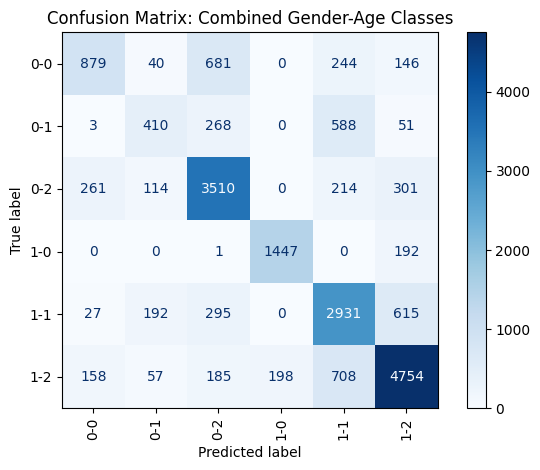
\includegraphics[width=1\linewidth]{images/lr/cm-reduced-data.png}
    \caption{Confusion Matrix (liblinear + L1)}
    \label{fig:cm-liblinear-l1}
\end{figure}
This shows that utilising a model, using different hyper-parameters and solvers is not enough. Another experiment is to select certain features via correlation which is explored in the next section. 
\subsection{Feature selection and correlation}
Earlier we discussed the correlation matrix, putting that to use is extremely critical for logistic regression since it dropping features will be key for the model to perform better.
The original correlation matrix in Figure~\ref{fig:correlation-matrix} showed several clusters particular around features such as velocity and gyroscope data, which can introduce multicollinearity and stop the model to be interpretable especially in terms of its coefficients. The dropped features were \texttt{[ax\_rms, ay\_rms, gx\_rms, gy\_rms, gz\_rms, a\_ma, a\_mean, g\_fft, g\_psdx, g\_entropy, holdRacketHanded\footnote{Note that we previously discussed how holdRacketHanded was an extremely imbalanced feature in Figure~\ref{fig:stacked-hand-results} and now it has been dropped.}]} 

\begin{figure}[H]
    \centering
    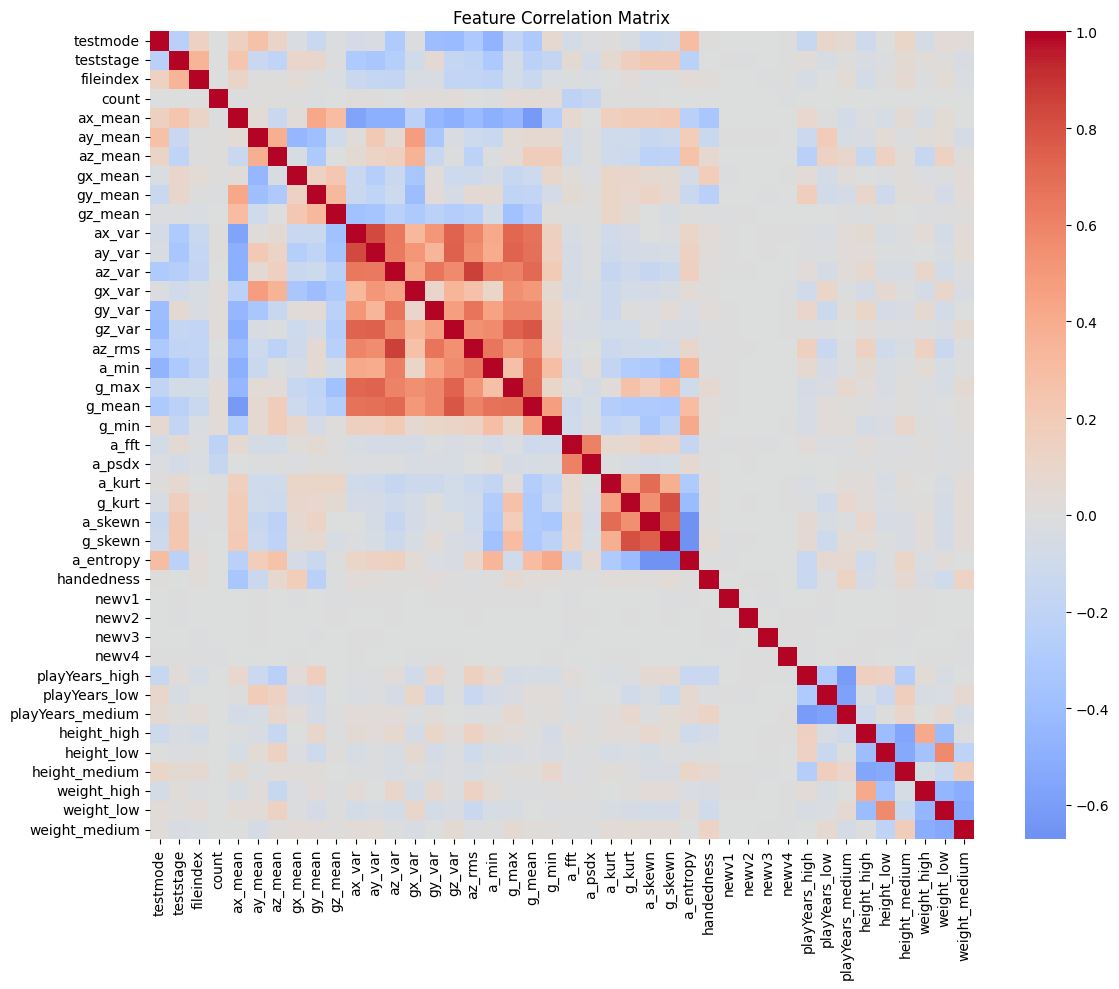
\includegraphics[width=1\linewidth]{images/lr/reduced-correlation-matrix.png}
    \caption{Reduced correlation matrix}
    \label{fig:reduced-correlation-matrix}
\end{figure}
After applying a correlation threshold of $p=0.9$, the new correlation matrix shows a much clearer relationship and the big cluster has now been reduced to a smaller cluster with only one diagonal instead of 3 diagonal lines. 
Finally we train out model again, but this time, we change the train-test-split to 90-10\%. Table~7 outlines the new accuracy for our logistic model. This time out accuracy is 73.2\% which is a 1.65\% increase. 
\begin{table}[H]
\centering
\caption{Classification Report for Logistic Regression (LIBLINEAR + L1)}
\resizebox{\linewidth}{!}{%
\begin{tabular}{|c|c|c|c|c|}
\hline
\textbf{Class} & \textbf{Precision} & \textbf{Recall} & \textbf{F1-Score} & \textbf{Support} \\
\hline
0 & 0.655 & 0.444 & 0.529 & 1990 \\
1 & 0.615 & 0.403 & 0.487 & 1320 \\
2 & 0.729 & 0.804 & 0.764 & 4400 \\
3 & 0.890 & 0.891 & 0.891 & 1640 \\
4 & 0.643 & 0.750 & 0.692 & 4060 \\
5 & 0.794 & 0.790 & 0.792 & 6060 \\
\hline
\textbf{Accuracy} & \multicolumn{4}{c|}{0.732} \\
\textbf{Macro Avg} & 0.721 & 0.680 & 0.693 & 19470 \\
\textbf{Weighted Avg} & 0.730 & 0.732 & 0.726 & 19470 \\
\hline
\end{tabular}
}
\label{tab:logreg-classification-report}
\end{table}
It seems to be doing well on class 3 and class 5 but performs poorly on class 0 and 1. We can also see that the support for class 0 and 1 are significantly less compared to class 3 and 5 which have higher than 4000 samples. The reason why class 3 and 5 are high-performing classes is due to the fact that logistic regression relies on learning class-specific weights using the available data. This multi-classification logistic model uses SoftMax which will inherently favour majority classes. The recall for class 0 and 1 is notably low indicating that the model failed to correctly identify more than half of the actual instances from these classes.
\begin{figure}[H]
    \centering
    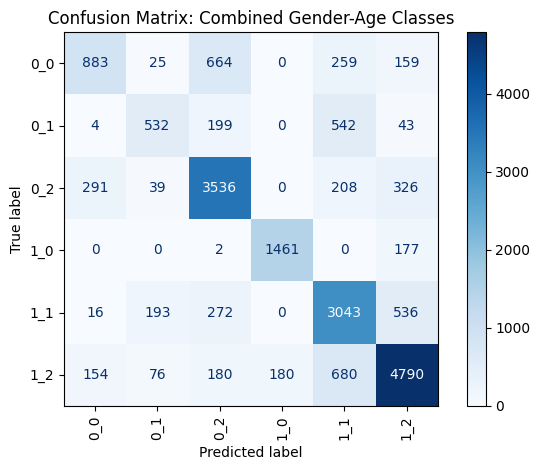
\includegraphics[width=1\linewidth]{images/lr/cm-liblinear-l1-normal-training.png}
    \caption{Confusion Matrix (features dropped)}
    \label{fig:cm-reduced-data}
\end{figure}
Nonetheless comparing Figure~\ref{fig:cm-liblinear-l1} with Figure~\ref{fig:cm-reduced-data}, we can see the increase of TPR across the diagonal. This shows that feature correlation from the dataset does have an impact on the accuracy of the model but in this experiment, it's not significant.
\begin{figure}[H]
    \centering
    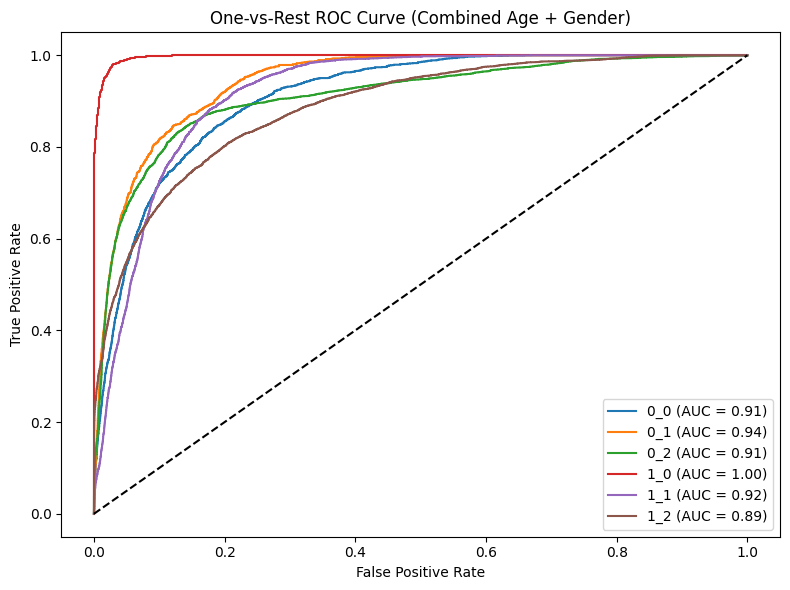
\includegraphics[width=1\linewidth]{images/lr/roc-liblinear-l1-normal-training.png}
    \caption{ROC (features dropped)}
    \label{fig:roc-reduced-data}
\end{figure}
For a much deeper inspection, The ROC shows strong class separation with AUC score above 0.88 for all classes. Class 1-0 stands out with an AUC of 1.00, which indicates flawless ranking for that particular class. class (1-2) shows the lowest score of 0.89. Despite high AUC values, these results must be interpreted alongside recall and accuracy, as high ranking performance does not always translate to correct predictions in a one-vs-rest strategy. Inspecting the false positive rate, we can see that it's significantly higher KNN's ROC curve in Figure~\ref{fig:knn-roc}.
\subsubsection{Cross validation on reduced correlation}
\begin{figure}[H]
    \centering
    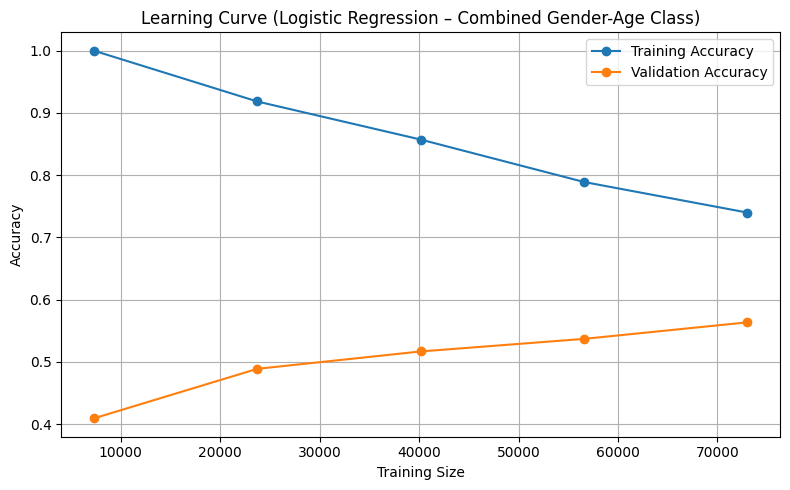
\includegraphics[width=1\linewidth]{images/lr/cross-validation - reduced.png}
    \caption{Learning curve (features dropped)}
    \label{fig:lr-learning-curve}
\end{figure}
To find the true capabilities of the model, we cross-validate with a stratified 4-fold with the liblinear solver and L2 regularisation on the reduced low-correlation feature dataset, which initially illustrates a high variance with the training performance being 100\%. As the training sizes gets larger, we can see the generalisation gap getting smaller and smaller in Figure~\ref{fig:lr-learning-curve}, with the training accuracy decreasing and validation increasing, showing moderate bias and some variance plateauing around $E_{hold-out}=57$\%. This shows on average, the model struggles due to the complexity and overlap of class boundaries in the feature space, especially for minority classes. The model is not overfitting nor underfitting, it assumes a linear relationship between features and log-odds of classification, which might be too simplistic for capturing the nuanced decision surfaces (non-linear features) needed to separate six combined gender-age classes. Furthermore, we understand that switching from a non-parametric model (KNN) to a parametric model such as logistic regression that has the capability to learn weights and tune different hyperparameters, does not necessarily make a better model nor achieve a higher accuracy due to the mechanics of the individual model and loss functions used.

\clearpage
\section{Model 3: Support Vector Machine (SVM)}
To address the limitations of logistic regression, we look at kernel based methods where we can increase the dimensionality of the model to capture much more complex patterns in the data.

\subsection{Kernel and regularisation exploration}
For experimentation purposes through repeated trials with varying hyper parameters and kernels, we will see how the support vector classification works with the learning of the dataset. 
First we experiment with two kernels that are not generally used in practice for our dataset. Given we have non-linear features, we experiment and use the linear kernel $\kappa(\mathbf{x},\mathbf{x'}) = \mathbf{x}^\top \mathbf{x'}$ to see how well it performs. The sigmoid kernel $\kappa(\mathbf{x}, \mathbf{x}') = \tanh\left(a \mathbf{x}^\top \mathbf{x}' + b\right)$ which introduces non-linear decision boundaries through the tanh function will also be utilised. We foresee sigmoid will output the linear kernel depending on the regularisation $C$ parameter.

Furthermore, we train with our reduced correlated data with previous conditions as other models explored above and, we train our SVC with our regularisation parameter $C$ ranging from $0.1,1,5$. We observe that our linear kernel performs much better than sigmoid even though we have non-linear features and we validate this using mathematical reasoning.

\begin{figure}[H]
    \centering
    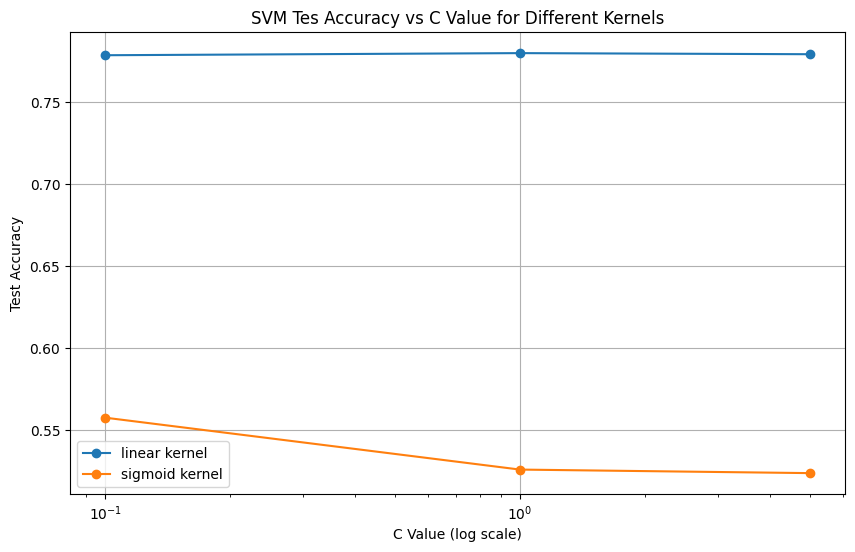
\includegraphics[width=1\linewidth]{images/svm/svm-linear-vs-kernel-and-regularisation.png}
    \caption{Linear vs Sigmoid Kernel ($C$=0.1,1,5)}
    \label{fig:svm-kernels}
\end{figure}
Figure~\ref{fig:svm-kernels} shows the performance of both kernels. We have specifically chosen two different kernels, where they aren't ideal due to their mechanics and mathematical expectations. If the kernel $\kappa$ is not positive semi-definite then this means that our eigenvalues can be complex and non-real. Sigmoid does not always guarantee a positive semi-definite matrix $X$, and the parameters $a$ and $b$ have to be carefully tuned, which cannot be directly done in \texttt{scikit-learn}'s API. This makes it difficult to directly create a hyperplane with less support vectors resulting with an initial accuracy of 56\%. SVC struggles with learning features and drops its accuracy down from $C=0.1$ to $C=1$ and stabilises with $C$=5.

In comparison, the linear kernel was originally thought to not be an ideal choice, however, it seems that it was able to linearly separate the features linearly (regardless of $C$) even though features are non-linear. Let's remember that the kernel trick allows for a hidden $\mathbf{\phi}(x)^T \mathbf{\phi}(x')$ function to have a large $d$ value which allows for high dimensional data. Additionally, the linear kernel guarantees a positive semi-positive kernel, which explains why it was able to generalise pretty well, averaging an accuracy of 78\% which is 22\% better than sigmoid and 6.5\% better than our original highly-correlated logistic regression model. Our linear kernel allows for an eigenvalue $\lambda >= 0$ and we also have a symmetric matrix $K$ which helps the model create a linear hyperplane to separate complex data reasonably well, especially with enough support vectors.

\subsection{Evaluation Metrics and Results}
\begin{figure}[H]
    \centering
    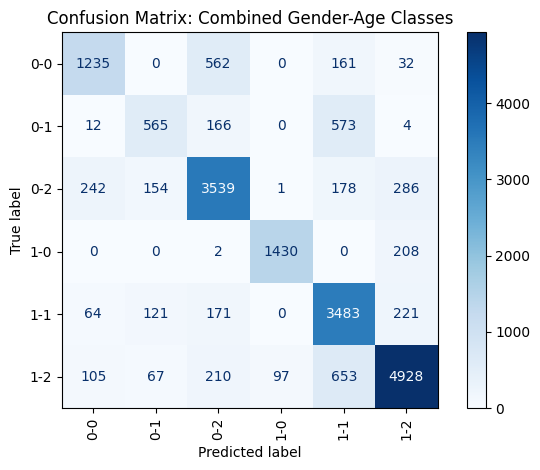
\includegraphics[width=1\linewidth]{images/svm/svm-cm-linear-vs-kernel-and-regularisation.png}
    \caption{SVC Confusion matrix (linear kernel)}
    \label{fig:svm-cm-kernels}
\end{figure}

Figure~\ref{fig:svm-cm-kernels}, shows good generalisation, with the number of true positives across the diagonal line. The model classifiers much better than logistic regression, and it's classifying class (0-2) almost as well as logistic regression but does significantly better with classes with more data such as class (1-2).
\begin{table}[H]
\centering
\caption{Classification Report (linear kernel)}
\resizebox{\linewidth}{!}{%
\begin{tabular}{|c|c|c|c|c|}
\hline
\textbf{Class} & \textbf{Precision} & \textbf{Recall} & \textbf{F1-Score} & \textbf{Support} \\
\hline
0 & 0.74 & 0.62 & 0.68 & 1990 \\
1 & 0.62 & 0.43 & 0.51 & 1320 \\
2 & 0.76 & 0.80 & 0.78 & 4400 \\
3 & 0.94 & 0.87 & 0.90 & 1640 \\
4 & 0.69 & 0.86 & 0.76 & 4060 \\
5 & 0.87 & 0.81 & 0.84 & 6060 \\
\hline
\textbf{Accuracy} & \multicolumn{4}{c|}{0.780} \\
\textbf{Macro Avg} & 0.77 & 0.73 & 0.75 & 19470 \\
\textbf{Weighted Avg} & 0.78 & 0.78 & 0.78 & 19470 \\
\hline
\end{tabular}
}
\label{tab:classification-77-accuracy}
\end{table}
A low recall of 43\% from class 1 indicates that the SVC suffers from class imbalance and limited flexibility. While the linear kernel is computationally efficient and works well with a high $d$, its inability to capture non-linear boundaries limits its performance on complex imbalanced classes for our gender-age problem. 

\begin{figure}[H]
    \centering
    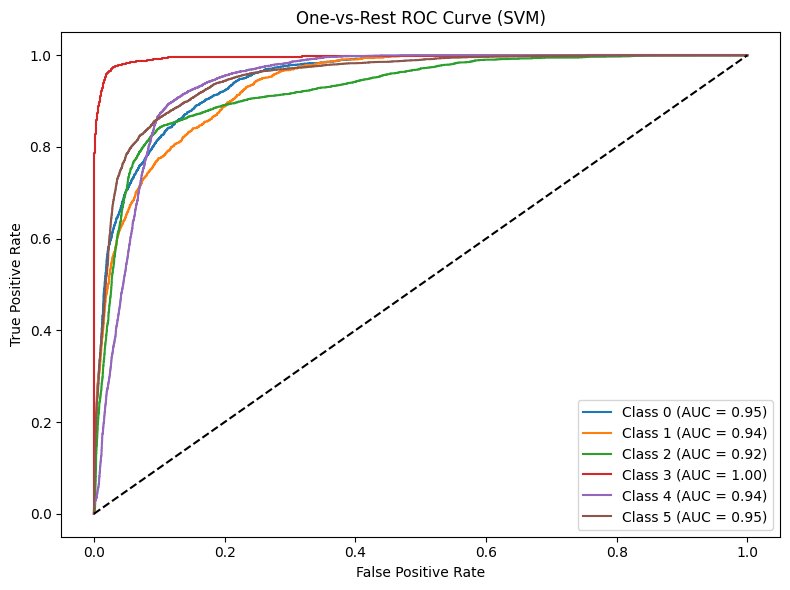
\includegraphics[width=1\linewidth]{images/svm/svm-roc-linear-vs-kernel-and-regularisation.png}
    \caption{SVC ROC Curve}
    \label{fig:svm-roc-kernels}
\end{figure}

The ROC curve very well confirms that the linear SVM ranks class predictions well, achieving high AUCs across all classes. However, its lower recall for minority classes as discussed in the Table~\ref{tab:classification-77-accuracy} suggests that while the model distinguishes classes effectively in terms of their probability scores, it still struggles to make correct hard classifications under the default decision threshold.
We conclude that while the linear kernel achieves a decent accuracy of 78\%, it's not considered the best.

\subsection{More experiments - Polynomial Kernel}

This time we will explore deeper with a different kernel which is also positive semi-definite for favourable reasons - Polynomial kernel $\kappa(\mathbf{x}, \mathbf{x}') = (c + \mathbf{}{x}^\top \mathbf{}{x}')^{d - 1}$. We have the same conditions as before primarily because we would like to analyse how our model behaves with different kernels and regularisation parameters.

\begin{table}[H]
\centering
\caption{Classification Report (Polynomial kernel)}
\resizebox{\linewidth}{!}{%
\begin{tabular}{|c|c|c|c|c|}
\hline
\textbf{Class} & \textbf{Precision} & \textbf{Recall} & \textbf{F1-Score} & \textbf{Support} \\
\hline
0 & 0.929 & 0.882 & 0.905 & 1990 \\
1 & 0.963 & 0.924 & 0.943 & 1320 \\
2 & 0.950 & 0.939 & 0.945 & 4400 \\
3 & 0.981 & 0.958 & 0.969 & 1640 \\
4 & 0.913 & 0.956 & 0.934 & 4060 \\
5 & 0.946 & 0.954 & 0.950 & 6060 \\
\hline
\textbf{Accuracy} & \multicolumn{4}{c|}{0.942} \\
\textbf{Macro Avg} & 0.947 & 0.936 & 0.941 & 19470 \\
\textbf{Weighted Avg} & 0.942 & 0.942 & 0.942 & 19470 \\
\hline
\end{tabular}
}
\label{tab:svm-poly-report}
\end{table}
Table~\ref{tab:svm-poly-report} demonstrates and accuracy of 91\% for all precision which means that the polynomial kernel was able to determine most of the classes by that metric. All classes had a minimum recall of 88.2\% and a high recall of 95.8\% indicating low variance and, how often it's able to identify all relevant positive instances within the dataset. Moreover it has achieved a training accuracy of 94.96\% and testing accuracy of 94.2\%, which is a massive improvement from previous discussed kernels. 

\begin{figure}[H]
    \centering
    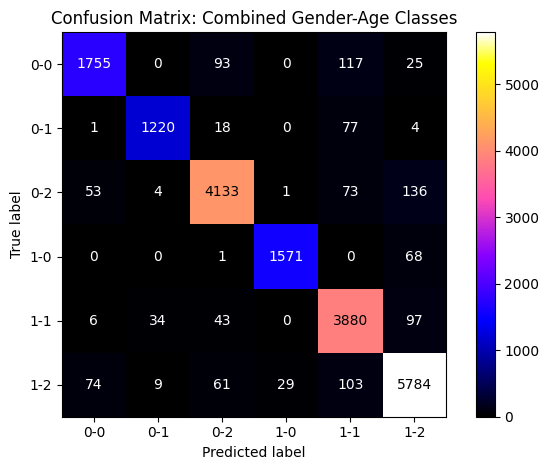
\includegraphics[width=1\linewidth]{images/svm/svm-cm-poly.png}
    \caption{SVC Confusion matrix (Poly Kernel)}
    \label{fig:svm-poly-cm}
\end{figure}
Utilising the polynomial kernel introduces non-linear boundaries by modelling certain feature interactions through polynomial terms. Unlike the linear kernel which can only create linear hyperplanes, the polynomial kernel allows our SVC to learn complex relationships between features especially where classes are defined by subtle combinations of demographic (age-gender) and motion-based features. The model was able to capture non-linear features such as swing kinetics, angular velocity etc.. when linear kernel couldn't.
Figure~\ref{fig:svm-poly-cm} should visually illustrate how much more accurate the model is compared to previous experimentation. Even though it has a high \texttt{TPR}, there is still some confusion between classes such as middle-aged male (1-1) and older male (1-2).
\begin{figure}[H]
    \centering
    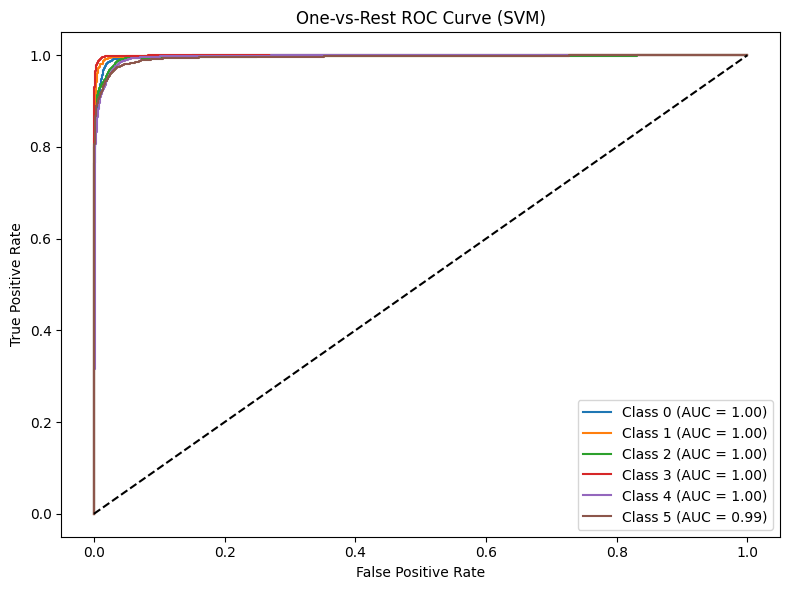
\includegraphics[width=1\linewidth]{images/svm/svm-poly-roc.png}
    \caption{SVM ROC Curve (Poly kernel)}
    \label{fig:svm-roc-poly}
\end{figure}
To further evaluate how well the classes are being separated on a polynomial scale, we analyse an ROC curve. Figure~\ref{fig:svm-roc-poly} reveals almost perfect gender-age discrimination across all six classes, with AUC values of 1.0 except for class 5. This confirms  SVC's ability to accurately rank class probabilities, which validates the clear effectiveness of the polynomial kernel.
he ROC curve for the polynomial SVM reveals near-perfect discrimination across all six classes, with AUC values of 1.00 for five classes and 0.99 for the sixth. This confirms the model’s ability to accurately rank class membership probabilities, validating the effectiveness of the polynomial kernel in capturing the non-linear structure of the gender-age classification task. The steep ROC curves and the minimal deviation from the top-left corner shows how well SVC performs with the polynomial kernel.

This summarises the power of support vector machines along as the right kernel has been selected in relation to the complexity and structure of the dataset. In this case, the polynomial kernel is the most preferred one, not necessarily because of its high accuracy, but primarily because it's more suitable to learning non-linear patterns and it's distinct properties that allows matrices to have real eigenvalues $\lambda$.
\section{Conclusion}
We will conclude by presenting a strong analysis of the models explored.
\subsection{Bias variance trade off}
Logistic Regression has moderate bias and low variance, and under fits to the training data and is unable to capture features under normal training and cross validation. With cross validation, KNN has low bias and high variance, which means that it first the training data very well, but suffers from generalisation issues due to sensitivity to data noise and class imbalance. Otherwise, (without cross-validation), KNN works remarkably well, with low bias and low variance. For SVC, with the polynomial kernel, we have low bias and low variance as proven in the Table~\ref{tab:svm-poly-report}.
\subsection{Comparative Analysis}
The results show that non-linear class boundaries are crucial for this task which is why KNN originally achieved an high accuracy (with $k=3$) of 96\% and SVM with the polynomial kernel performing at 94.2\% which are highly close. KNN originally worked very well because of its distance mechanism, while SVC makes use of the hinge loss, where in our case we had less support vectors $\alpha_i$ influencing the decision boundaries. Logistic regression is last in terms of performance because it assumes strong linear relationship of which the dataset is incapable of providing as proven by low predictions accuracies. Most of its coefficients were very negative demonstrating its ability to generalise well. Overall, the combined label gender-age was able to be classified accurately with some of these models showcasing that there are critical features that strictly determine the differences between and young and older people including gender. We can empirically say that our models such as SVM, was able to still differentiate between men and women primarily because of the difference in biological factors that play out with the recorded  acceleration and angular velocity features.
\subsection{Insights on applied models and suggestions for future experimentation}
For future experiments, perhaps a stronger assumption in relevance to the distribution of the data should have been made, such as assuming specific different distributions of subsets of features that follow similar distributions.

A distance metric, we could have used in cross validation for KNN, includes Manhattan and Mahalanobis distance, which accounts for feature distributions and correlation.

For a more comprehensive evaluation of SVM, it would be good to experiment with the radial basis function which is mostly used by machine leaning engineers in SVM configuration for complex datasets. The reason we do not in this paper is to understand SVM's true capabilities when restricted to less kernels. Other examples would include the Matérn family of kernels, which again are positive semi-definite. The reason we stress so much for this property is so that $\mathbf{}{K}(\mathbf{X},\mathbf{X})$ is invertible, otherwise it's very difficult to compute predictions.

Even though Logistic regression was not the strongest model, it did get an accuracy of 71.55\%, which illuminates the idea of employing a bagging or boosting model, such as AdaBoost which can help reduce both bias and variance present.

\printbibliography

% \clearpage  % or \newpage
\appendix
\section*{Appendix}



\begin{equation}{\dfrac 1 n} \sum^n_{i=1}  \underbrace{\ln ({1+e^{-y_i \theta^\top x_i}})}_{\text{Logistic Loss \ } L(x_i, y_i, \theta_i)}\label{eq:logistic-loss}
\end{equation}

\begin{table}[H]
\centering
\footnotesize
\caption{LIBLINEAR + L2 (Rounded Coefficients)}
\begin{tabular}{|c|p{6.5cm}|}
\hline
\textbf{Class} & \textbf{Top Features (Coefficient)} \\
\hline
0 & \texttt{height\_high} (-3.02), \texttt{height\_medium} (1.75) \\
1 & \texttt{ay\_rms} (-3.37), \texttt{playYears\_high} (-2.33) \\
2 & \texttt{a\_mean} (2.19), \texttt{ax\_rms} (-1.96) \\
3 & \texttt{height\_high} (5.32), \texttt{height\_low} (-3.83) \\
4 & \texttt{playYears\_high} (-2.36), \texttt{ax\_rms} (1.96) \\
5 & \texttt{ax\_mean} (-1.72), \texttt{a\_mean} (-1.62) \\
\hline
\end{tabular}
\label{tab:logreg-liblinear-l2}
\end{table}

\begin{table}[H]
\centering
\footnotesize
\caption{LBFGS + L2 (Rounded Coefficients)}
\begin{tabular}{|c|p{6.5cm}|}
\hline
\textbf{Class} & \textbf{Top Features (Coefficient)} \\
\hline
0 & \texttt{height\_high} (-3.38), \texttt{height\_medium} (1.94) \\
1 & \texttt{ay\_rms} (-3.25), \texttt{playYears\_high} (-2.77) \\
2 & \texttt{a\_mean} (2.21), \texttt{ax\_rms} (-1.96) \\
3 & \texttt{height\_high} (6.77), \texttt{height\_low} (-4.29) \\
4 & \texttt{playYears\_high} (-2.60), \texttt{ax\_rms} (1.95) \\
5 & \texttt{ax\_mean} (-1.72), \texttt{a\_mean} (-1.53) \\
\hline
\end{tabular}
\label{tab:logreg-lbfgs-l2}
\end{table}

\begin{figure}[H]
    \centering
    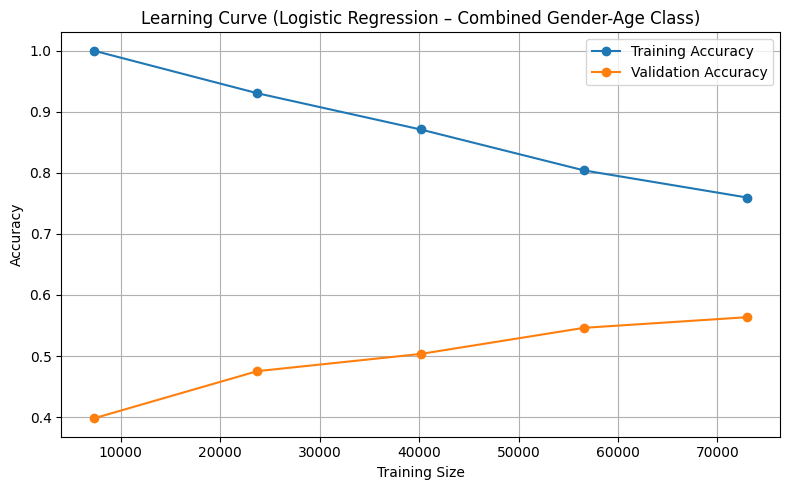
\includegraphics[width=1\linewidth]{images/lr/cross-validation - normal.png}
    \caption{Learning curve for Logistic Regression}
    \label{fig:reduced-learning-curve}
\end{figure}

\begin{figure}[H]
    \centering
    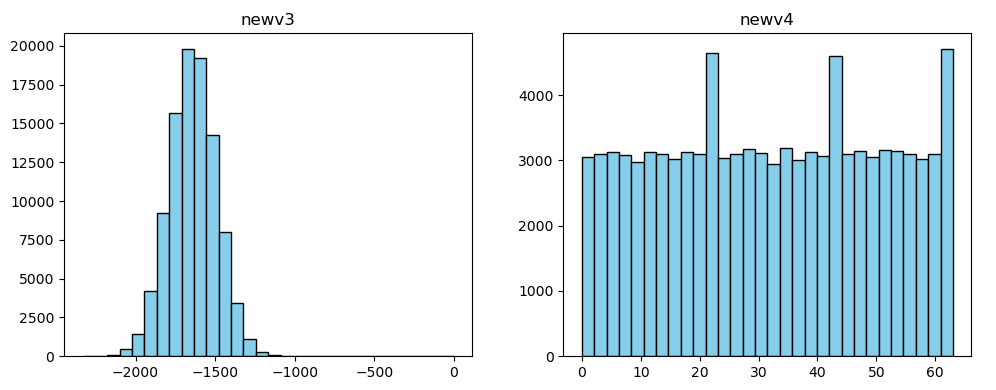
\includegraphics[width=0.85\linewidth]{images/distribution_3.png}
    \caption{Distributions of features (1 of 4).}
    \label{fig:distribution-3}
\end{figure}

\begin{figure}[H]
    \centering
    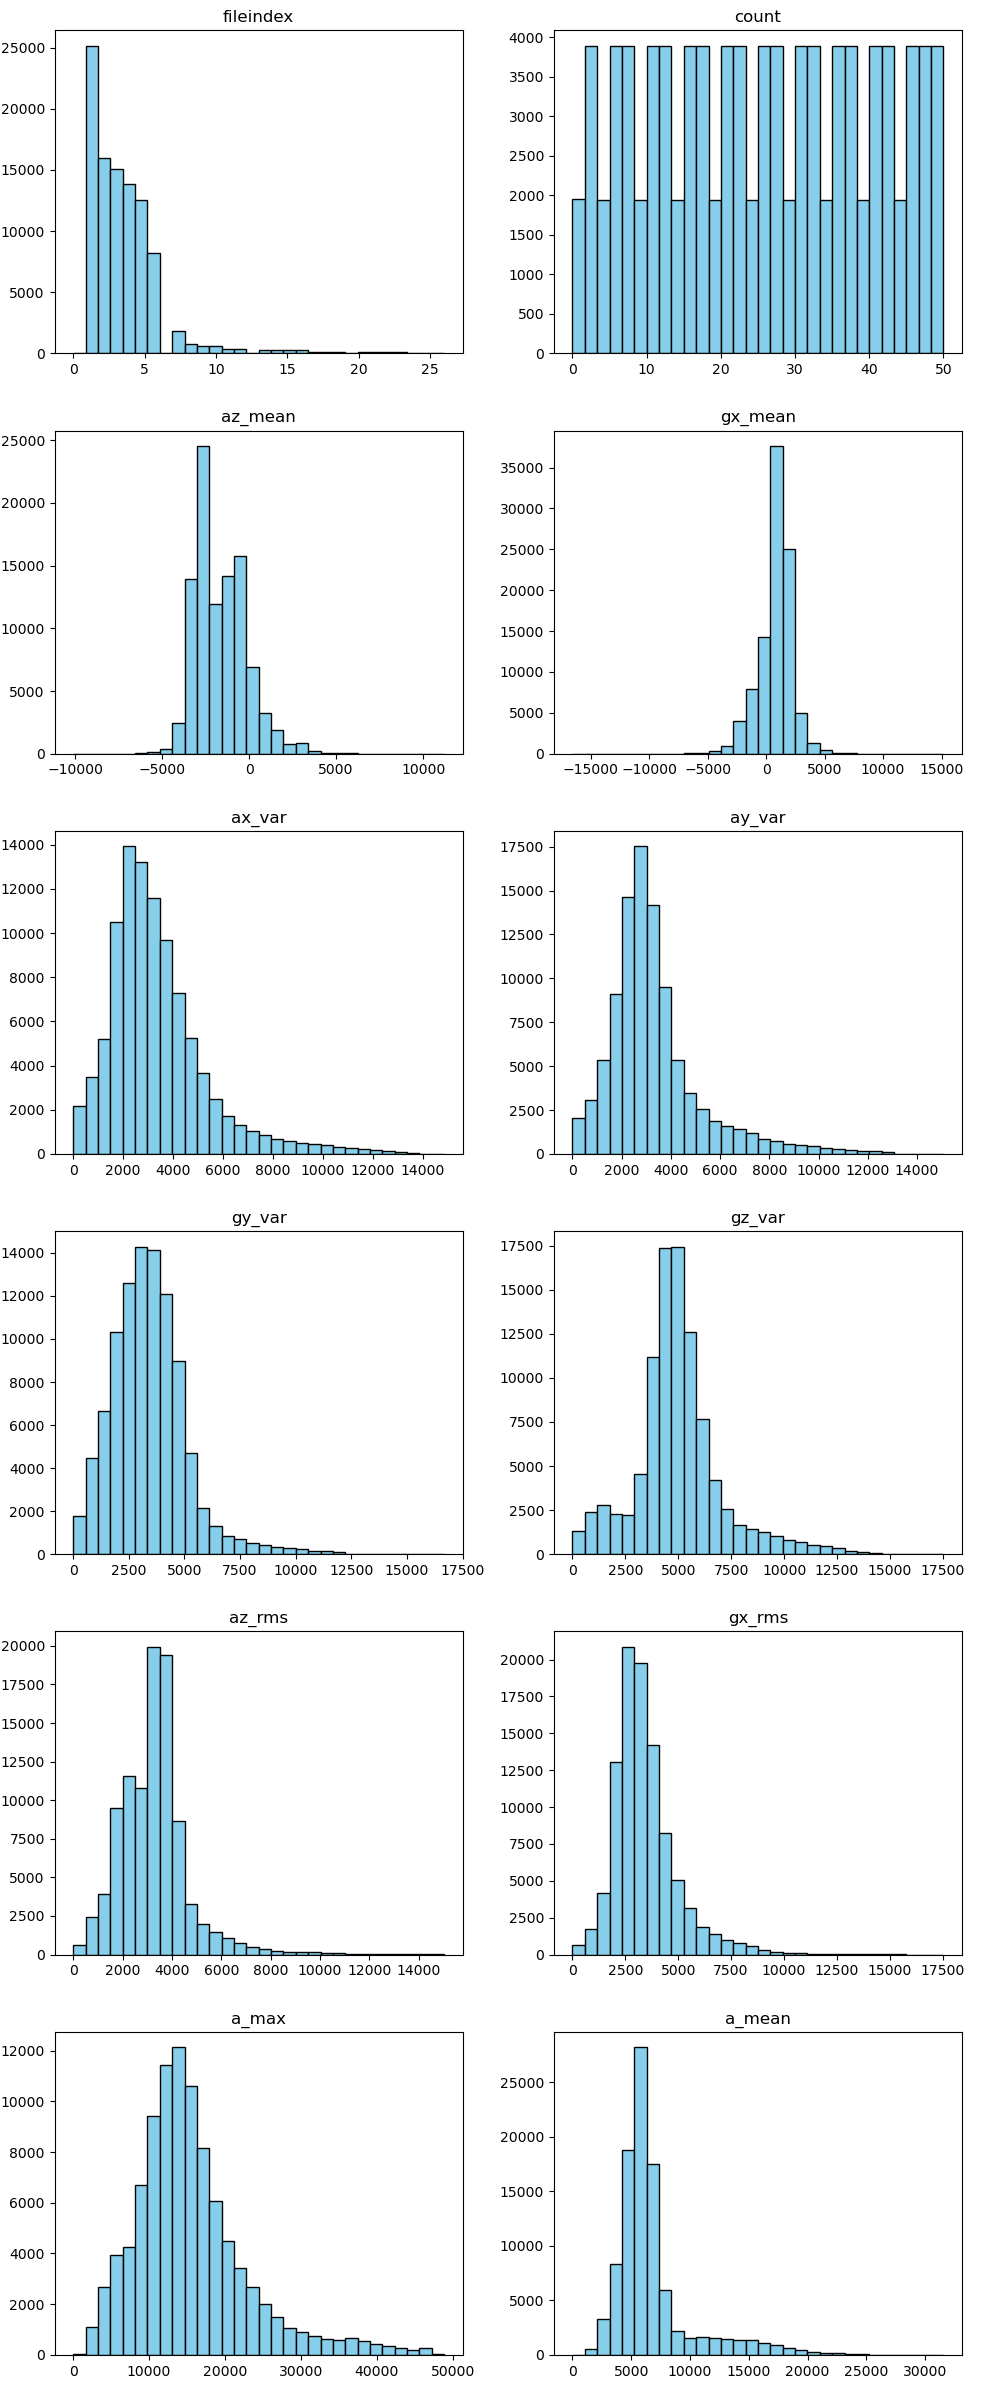
\includegraphics[width=0.85\linewidth, height=0.4\textheight]{images/distribution_2_1.png}
    \caption{Distributions of features (2 of 4).}
    \label{fig:distribution-2-1}
\end{figure}

\begin{figure}[H]
    \centering
    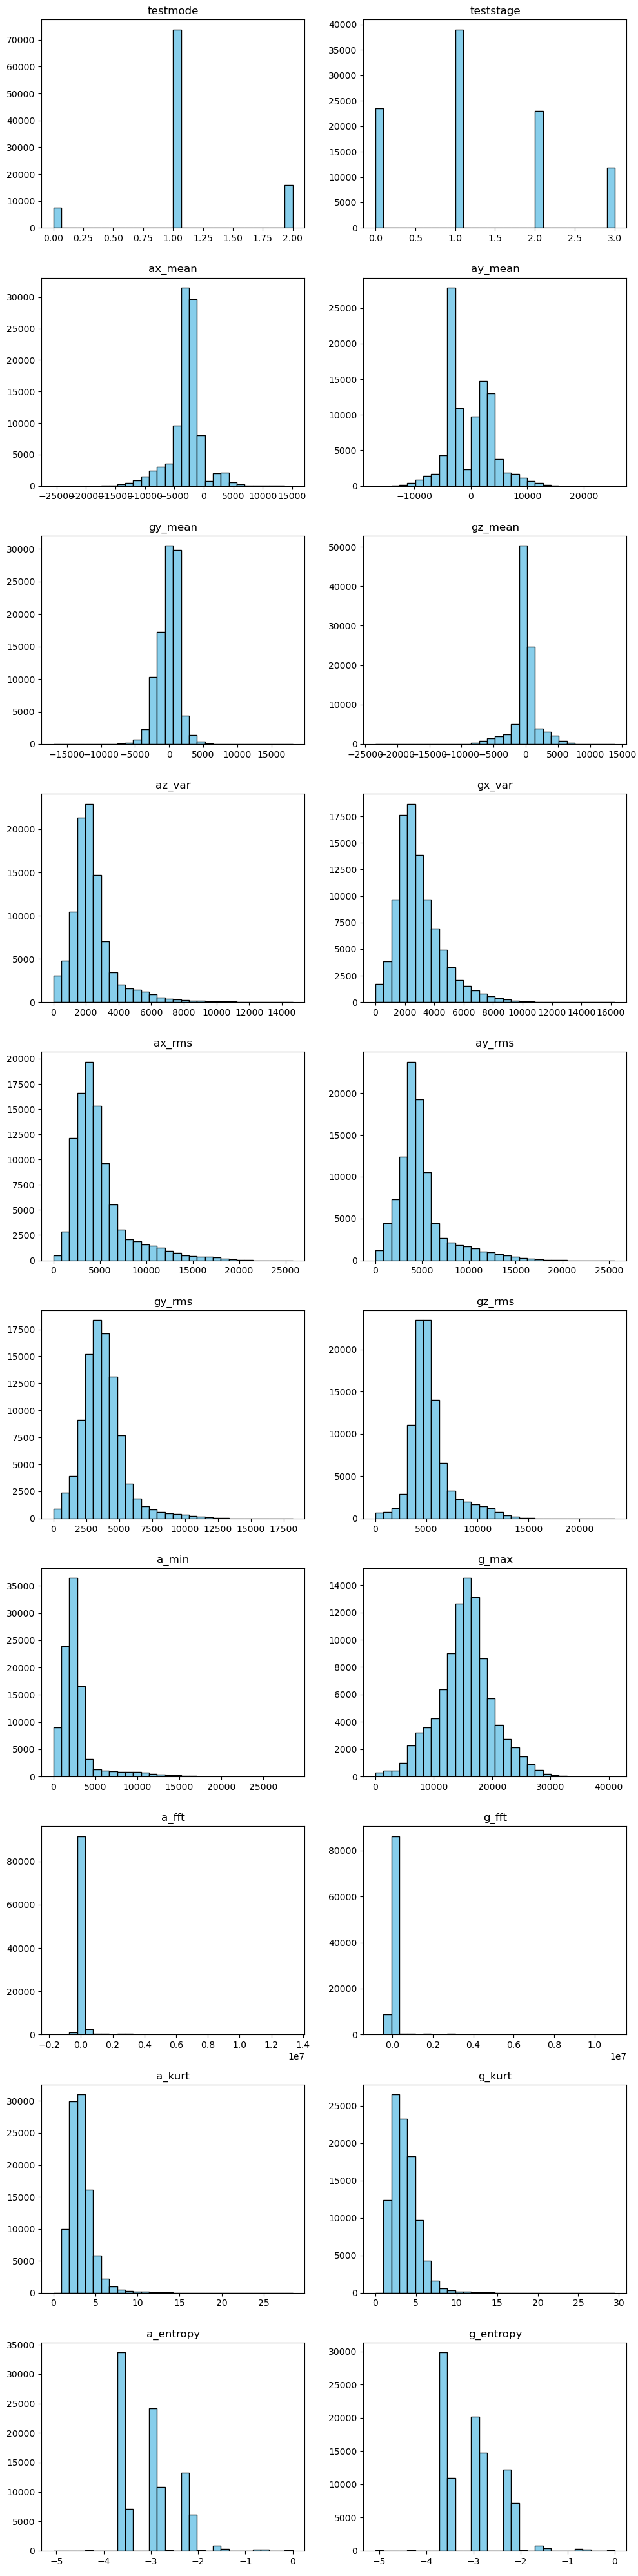
\includegraphics[width=0.85\linewidth, height=0.9\textheight]{images/distribution_1.png}
    \caption{Distributions of features (3 of 4).}
    \label{fig:distribution-1}
\end{figure}

\begin{figure}[H]
    \centering
    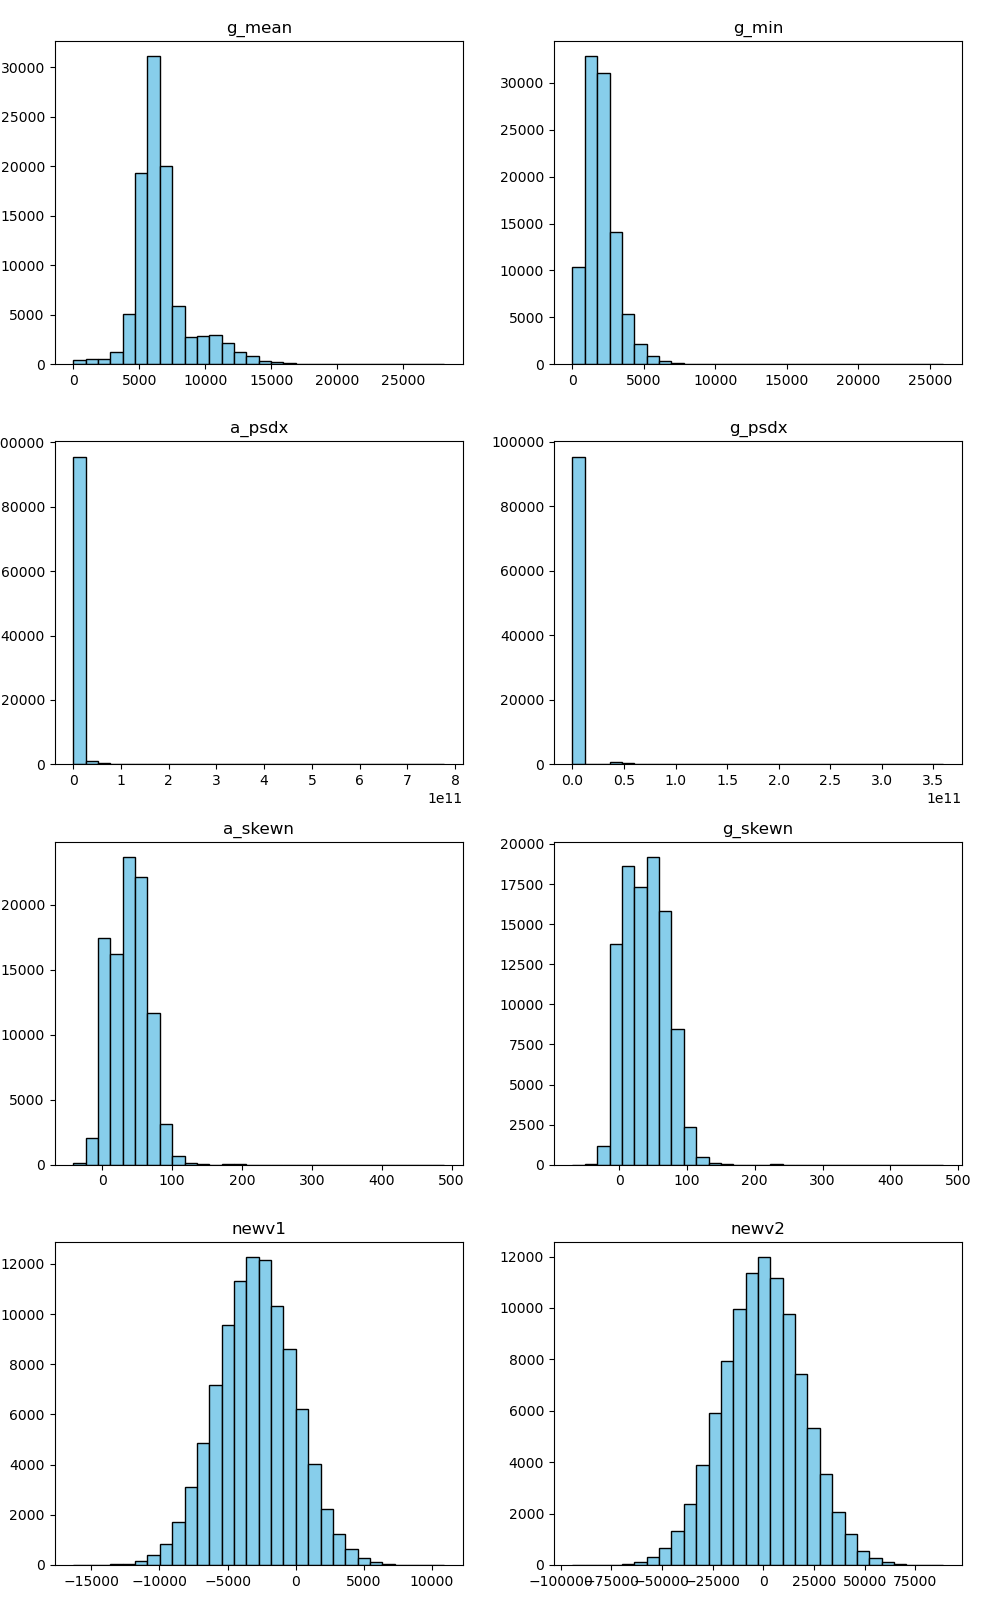
\includegraphics[width=0.85\linewidth, height=0.4\textheight]{images/distribution_2.png}
    \caption{Distributions of features (4 of 4).}
    \label{fig:distribution-2-2}
\end{figure}

\end{document}

